\section{How HMMER builds profile HMMs from alignments}

This section walks you through the steps of building a model from a
multiple sequence alignment, in gory detail. You have a fair amount of
control over many of these steps, using options to the \prog{hmmbuild}
program.

We'll start with a description of the ``Plan 7'' profile HMM
architecture used by HMMER, and the philosophy behind it. It differs
in small but important ways from the original Krogh/Haussler
architecture. Specifically, Plan 7 is a fully probabilistic model of
both local and global profile alignment. It distinguishes between
\emph{data-dependent} probabilities that are learned from a query
multiple alignment and \emph{algorithm-dependent} probabilities that
are configured by choosing a particular alignment mode.

\subsection{The Plan 7 profile HMM architecture}

HMMER uses a profile HMM architecture called Plan 7 that is somewhat
more complex than the original profile HMM architecture introduced by
Krogh, Haussler, and coworkers \citep{Krogh94}.

The heart of a profile HMM is a linear set of match (M) states, one
per consensus column in the multiple alignment. Each M state emits
(aligns to) a single residue, with a probability score that is
determined by the frequency that residues have been observed in the
corresponding column of the multiple alignment. Each match state
therefore carries a vector of 20 probabilities, for scoring the 20
amino acids.

Some analysis approaches, including BLOCKS \citep{Henikoff94}, are
essentially equivalent to a profile HMM composed only of M states.
These methods are called \emph{weight matrices} or
\emph{position-specific score matrices} (PSSMs); they look for
\emph{ungapped} alignments to a consensus.

\begin{figure}[t]
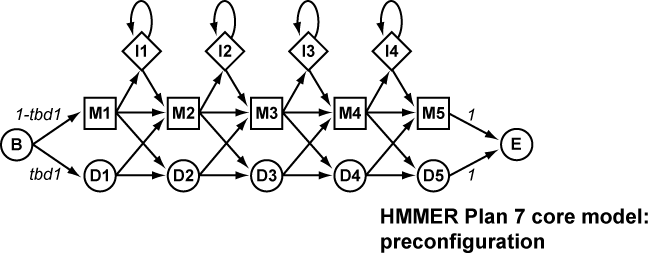
\includegraphics{plan7-core}
\caption{\textit{The core of the Plan7 architecture. Squares indicate
match states (modeling consensus positions in the alignment).
Diamonds indicate insert states (modeling insertions relative to
consensus) and special random sequence emitting states. Circles
indicate delete states (modeling deletions relative to consensus) and
special begin/end states. Arrows indicate state transitions. Every
match state and insert state also carries an emission probability
distribution, for the observable symbols (4 nucleotides or 20 amino
acids).}}
\end{figure}

A profile HMM is capable of modeling gapped alignments, e.g. including
insertions and deletions, which lets the software describe a complete
conserved domain (rather than just a small ungapped motif). Insertions
and deletions are modeled using (surprise!) insertion (I) states and
deletion (D) states. Each match state has an I and a D state
associated with it. HMMER calls a group of three states (M/D/I) at the
same consensus position in the alignment a ``node''.

These states are interconnected with arrows called \emph{state
transition probabilities}. The transitions are arranged so that at
each node, either the M state is used (and a residue is aligned and
scored) or the D state is used (and no residue is aligned, resulting
in a deletion-gap character, '-'). Insertions occur between nodes, and
I states have a self-transition, allowing one or more inserted
residues to occur between consensus columns. The transition to an I
state for the first inserted residue, followed by zero or more I
$\rightarrow$I self-transitions for each subsequent inserted residue,
is the probabilistic equivalent of the familiar gap-open and
gap-extend \emph{affine gap} penalty system, where one pays a
(usually) high cost for opening a gap and a (usually) lower cost for
extending it.

The model begins and ends with dummy non-emitting states, B and E.

This core section of the Plan 7 model, composed of M, D, and I nodes,
flanked by B and E states, is essentially a Krogh/Haussler profile
HMM.  This is the ``core model''. The core model controls the
\textit{data dependent} features of the model. All the probability
parameters in the main model are generally estimated from observed
frequencies of residues and transitions in a multiple sequence
alignment.

Unlike the original Krogh/Haussler and HMMER model architecture, Plan
7 has no D $\rightarrow$ I or I $\rightarrow$ D transitions. This
reduction from 9 to 7 transitions per node in the main model is one of
the origins of the name Plan 7. (The original Krogh/Haussler
architecture is called Plan 9 in parts of the HMMER source
code.)\footnote{The true origin of the codename is left undocumented,
as it reveals an inordinate fondness for bad science fiction
movies. Frighteningly, David Haussler understood immediately.}

\begin{figure}[t]
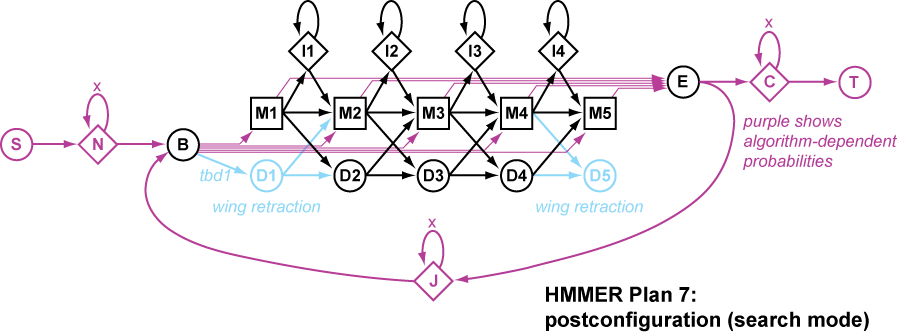
\includegraphics{plan7-search}
\caption{\textit{A complete Plan7 model, after configuration.}}
\end{figure}

The core model is augmented by five special states (S,N,C,T,J) and
additional state transition parameters to create the fully configured
Plan7 model. These additional states and parameters control
\textit{algorithm dependent} features of the model: e.g. how likely
the model is to generate various sorts of local or multihit
alignments. The algorithm dependent parameters are typically not
learned from data, but rather set externally by choosing a desired
alignment style.

In summary, the abbreviations for the states are as follows:

\begin{wideitem}
\item [\textbf{M$_x$}] Match state $x$.  Has $K$ emission probabilities.
\item [\textbf{D$_x$}] Delete state $x$. Non-emitter.
\item [\textbf{I$_x$}] Insert state $x$. Has $K$ emission probabilities.
\item [\textbf{S}]     Start state. Non-emitter.
\item [\textbf{N}]     N-terminal unaligned sequence state. 
    Emits \textit{on transition} with $K$ emission probabilities.
\item [\textbf{B}]     Begin state (for entering main model). Non-emitter.
\item [\textbf{E}]     End state (for exiting main model). Non-emitter.
\item [\textbf{C}]     C-terminal unaligned sequence state.
    Emits \textit{on transition} with $K$ emission probabilities.
\item [\textbf{J}]     Joining segment unaligned sequence state.
    Emits \textit{on transition} with $K$ emission probabilities.
\end{wideitem}

\subsubsection{the philosophy of Plan 7}

HMMs are \emph{generative probabilistic models}. Generative models
address a serious theoretical problem. To do correct statistical
inference, we need to be able to calculate a probability distribution
$P(S | M)$ for the probability of sequences $S$ given a model $M$, and
have this quantity sum to one over the ``space'' of all sequences.
But the number of possible different sequences $S$ is effectively
infinite, because they can be of any length. We can't just enumerate
this distribution, or we'd have to estimate an infinite number of
parameters. How do we make a \emph{finite} model of an \emph{infinite}
data space?  Generative models work by \emph{recursive} enumeration of
possible sequences from a finite set of rules -- rules that in an HMM
are represented by states, state transitions, and symbol emission
probabilities.

(In a profile HMM, the recursion is trivial: the self-transition
probability of the insert states, which allows insertions of any
length between two positions in the consensus. This simple model
implies a geometric distribution over insertion lengths -- as does any
linear or affine gap scoring system, in fact. Biologically, insertions
empirically follow a distribution with a longer tail, but more
realistic insertion models are computationally more expensive. The
marginal expected gain in performance is not thought to be worth the
extra computational effort.)

As described in \citep{Krogh94}, profile HMMs were originally
described as models of \emph{global alignment}: the sequence $S$ that
the model generates usually starts at the first match state and ends
at the last match state.

In real alignments of real biological sequences, global alignment is
rarely useful. A profile HMM is usually a model of a conserved domain,
not necessarily a model of a complete target sequence. A conserved
domain may be buried in a longer target sequence; there might be more
than one conserved domain in the target sequence; and maybe the target
sequence only contains a smaller fragment of the conserved domain. In
real applications, we prefer \emph{local alignment} algorithms, which
look for a high-scoring alignment between a subsequence of the target
sequence and a part of the query model. The common tools of sequence
analysis -- BLAST, FASTA, and Smith/Waterman alignment -- are all
local alignment algorithms.

It is straightforward to hack local alignment style algorithms around
the core Krogh/Haussler model of global alignment to a domain.  This
is what early versions of profile HMM software did, including
HMMER1. But some of the power of probabilistic modeling gets thrown
away; the resulting local alignment scores are no longer interpretable
as probabilities, because we have to introduce arbitrary
nonprobabilistic parameters for the local alignment (such as the usual
score of 0 for starting or ending a Smith/Waterman local alignment).

At least from a probabilistically purist perspective, it would be
sensible to revise the original Krogh/Haussler model to generate
\emph{complete} target sequences -- that is, modeling one or more
(possibly incomplete) matches to the domain model, and also modeling
the \emph{unaligned} sequence in the target. This is what Plan 7 does.

\subsubsection{the fully probabilistic ``local'' alignment models of Plan 7}

The Plan 7 architecture explicitly models the \emph{entire} target
sequence, regardless of how much of that sequence matches the main
model. \emph{All alignments to a Plan 7 model are ``global''
alignments:} a complete target sequence is aligned to a complete path
through the model from a start state (S) to the terminal state (T).
However, some (possibly most) of the sequence may be assigned to Plan
7 states (N,C,J) that generate nonhomologous, unaligned, ``random''
sequence that is not aligned to the main model.  Thus, the algorithm
dependent parts of the model control the \emph{apparent} locality of
the alignments.

Local alignments with respect to the sequence (i.e., allowing a match
to the main model anywhere internal to a longer sequence) are
controlled by the N and C states. If the N $\rightarrow$ N transition
is set to 0, alignments are constrained to have no unaligned
N-terminal sequence. Similarly, if the C $\rightarrow$ C transition is
set to 0, alignments are constrained to have no unaligned C-terminal
sequence.

Local alignments with respect to the model (i.e., allowing fragments
of the model to match the sequence) are controlled by B $\rightarrow$
M ``entry'' transitions and M $\rightarrow$ E ``exit'' transitions,
shown as dotted lines in the Plan 7 figure. Setting all entries but
the B $\rightarrow$ M$_1$ transition to 0 forces a partially
``global'' alignment in which all alignments to the main model must
start at the first match or delete state. Setting all exits to 0 but
the final M $\rightarrow$ E transition (which is always 1.0) forces a
partially global alignment in which all alignments to the main model
must end at the final match or delete state.

Multiple hit alignments are controlled by the E $\rightarrow$ J
transition and the J state. If the E $\rightarrow$ J transition is set
to 0, a sequence may only contain one domain (one alignment to the
main model). If it is nonzero, more than one domain per sequence can
be aligned to the main model. The J $\rightarrow$ J transition
controls the expected length of the intervening sequence between
domains; the lower this probability, the more clustered the domains
are expected to be.

\subsubsection{available alignment modes}

Because the alignment mode in Plan 7 is determined by the HMM
configuration, not by the search algorithm, you choose your alignment
style when you build the model -- not when you do the search.

The \prog{hmmbuild} program currently allows you to choose one of four
alignment modes, as follows. They are called \prog{hmmls},
\prog{hmmfs}, \prog{hmmsw}, and \prog{hmms} mode for historical
reasons -- these were the names of the corresponding search programs
in HMMER1.

\begin{wideitem}
\item [\emprog{hmmls}] This is like ``profile'' alignment or
``glocal'' alignment (as Waterman and others call it): global with
respect to the profile, and local with respect to sequence.  Multiple
nonoverlapping domains are allowed in the target sequence. $t_{NN}$
and $t_{CC}$ set to $t_{GG}$ from the null model (see below). $t_{EJ}$
set to 0.5. Internal entries and exits set to zero. This is the
default mode for HMMER.

\item [\emprog{hmmfs}] Multihit Smith/Waterman alignment: fully local
with respect to both the main model and the sequence; in addition,
multiple nonoverlapping alignments to more than one domain in the same
target sequence are allowed.  $t_{NN}$ and $t_{CC}$ set to $t_{GG}$
from the null model.  $t_{EJ}$ is set to 0.5.  Entry and exit
probabilities are set in a way such that all subsequences $i,j$ of the
model (starting at position $i$ and ending from position $j$) are
equiprobable (this is only roughly correct, as worded here; see source
code for detail). Activated by the \prog{hmmbuild -f} option.

\item [\emprog{hmmsw}] Smith/Waterman ``classic'' local alignment,
single best alignment per target. Same as \emprog{hmmfs} above, but
$t_{EJ}$ is set to zero. Activated by the \prog{hmmbuild -s} option.

\item [\emprog{hmms}] Needleman/Wunsch ``classic'' global alignment,
single best alignment per target. $t_{NN}$ and $t_{CC}$ set to
$t_{GG}$ from the null model. $t_{EJ}$ set to zero. Internal entries
and exits set to zero.  Activated by the \prog{hmmbuild -g} option.
\end{wideitem}

One advantage of Plan 7 is great flexibility in choosing an alignment
style. Complicated alignment styles are easily encoded in the model
parameters without changing the alignment algorithm.  For example, say
you wanted to model human L1 retrotransposon elements. Because of the
way L1 elements are inserted by reverse transcriptase (RVT), L1
elements tend to have a defined 3' end (RVT starts replication at the
same place in each new L1) but a ragged 5' end (RVT prematurely falls
off a new L1 in an unpredictable fashion). A specialized L1 model
could define non-zero internal entry probabilities and zero internal
exit probabilities to model this biological situation.

\begin{srefaq}{Why does Pfam distribute two sets of models, called
\prog{Pfam\_ls} and \prog{Pfam\_fs}?}  A disadvantage of Plan 7 is that
if you decide you want to do both local and global alignments, you
need two different models.  This wouldn't be too terrible, except for
the fact that the algorithm-dependent parameters strongly affect the
values of the $\mu$ and $\lambda$ parameters that E-value statistics
depend on. If the algorithm dependent parameters are changed, these
parameters are invalidated and the model needs to be recalibrated with
\prog{hmmcalibrate} -- but \prog{hmmcalibrate} is slow, so this can't
be done ``on the fly'' inside one of the search programs. It turns out
that ls mode is the most sensitive alignment mode, so long as a
complete domain alignment can be found; whereas fs mode is needed to
find domain fragments. Therefore Pfam is distributed with both sets of
models; for maximum detection ability of all homologies, both sets of
models have to be used.
\end{srefaq}

\subsection{Technical details on Plan 7 model configuration}

Skip this section unless you're interested in source code level detail.

In the figure of the fully configured Plan 7 architecture, you may
have noticed that the first and last delete states are greyed
out. Internally in HMMER, these delete states exist in the
``probability form'' of the model (when the model is being worked with
in every way except alignments) but they are carefully removed in the
``search form'' of the model (when the model is converted to log-odds
scores and used for alignments). This process is called ``wing
retraction'' in the code, by analogy to a swept-wing fighter changing
from a wings-out takeoff and landing configuration to a wings-back
configuration for high speed flight.

The technical problem that this is addressing is that the Plan 7 model
allows cycles through the J state. If a continuous nonemitting ``mute
cycle'' were allowed (J, B, D states, E, and back to J), dynamic
programming recursions would fail. This is why special mute states
like delete states must be handled carefully in HMM dynamic
programming algorithms \citep{Durbin98}. The easiest way to prevent a
mute cycle is to disallow them: make sure that the model must pass
through at least one match state per path through the main model.
Usually this can be done by breaking the chain somewhere and absorbing
the offending probability into a non-mute path.

Wing retraction involves folding the probabilities of the terminal
delete paths into the Plan 7 entry and exit probabilities. For
example, in wing retraction the ``algorithm dependent'' B
$\rightarrow$ M$_{3}$ entry probability is incremented by the
probability of the ``data dependent'' path B $\rightarrow$ D$_1$
$\rightarrow$ D$_2$ $\rightarrow$ M$_3$.

Wing retraction is done by the algorithm configuration routines. It is
only done for algorithms that allow beginning in or ending from a
delete state (global and glocal alignment modes). It is not done for
fully local Smith/Waterman modes (hmmfs and hmmsw modes) where the
algorithm-dependent begin and end distributions force entry and exit
only at match states.  Having the wing retraction step, rather than
{\em always} folding these probabilities together, is a design
decision, preserving a distinction between the ``algorithm dependent''
and ``data dependent'' parts of the model.

Because of wing retraction, the $D_1$ and $D_M$ states are never
accessed in dynamic programming alignment code. Their probabilities
are still kept in the model, so that the core model is remembered, and
a model can be ``deconfigured'' or reconfigured to a new algorithm
style. 

This leads to a peculiar technicality: the match state exit
transitions in a configured model can appear to be unnormalized,
because the exit transition from match state $k$ includes a dollop of
extra probability for the path that goes all-delete for the remainder
of the model ($k+1..M$). This is as should be, and everything balances
out, because exactly the sum of all those extra dollops of probability
get ignored when the DP algorithms ignore the final delete state.

\subsection{Parsing the residue information in input multiple sequence alignments}

\subsubsection{alphabet type: DNA or protein}

By default, the alphabet type (DNA or protein) is determined
automatically from the sequences in the alignment. This determination
primarily relies on the fact that some amino acid residues
(``EFIPQZ'') do not occur in DNA sequences, even in the IUPAC
degenerate code. Rarely, on small alignments, the autodetection may
resort to guesswork (and print a warning), or may fail altogether. You
can explicitly force the alphabet type using the \prog{--amino} or
\prog{--nucleic} option. 

\begin{srefaq}{Can HMMER make models of sequences other than DNA or
protein?} By default, HMMER requires DNA (RNA) or protein sequences.
But if you're willing to hack the code, the alphabet is configurable;
see the notes on the \prog{config.h} file,
page~\pageref{section:alphabet-config} in the installation section.
\end{srefaq}

\subsubsection{case insensitivity}

HMMER reads sequence residues in its input files in a
\emph{case-insensitive} manner.  (Internally, residues are handled
digitally, rather than alphabetically.) Other aspects of the file,
such as sequence names, preserve their case.

\begin{srefaq}{Why doesn't HMMER recognize Santa Cruz's SAM A2M format
properly?} HMMER can read an aligned FASTA format that is close, but
crucially not quite the Santa Cruz a2m format.  The real Santa Cruz
a2m format, used by the SAM profile HMM package, encodes match versus
insert column information in an upper vs. lower case convention in its
input files, and a - versus . convention for its gap characters.
Since HMMER digitizes residues case-insensitively, and treats
all gap characters identically in input files, this
information is lost. HMMER cannot currently read SAM a2m files
directly - even though the aligned fasta format is sometimes
called a2m! This is a historical misunderstanding of mine
about what the Santa Cruz format was; I thought it was simple...
\end{srefaq}

\subsubsection{handling of degenerate residue codes}

For amino acid sequences, HMMER accepts the standard IUPAC degeneracy
codes (BZX). It reads U (selenocysteine) as a valid amino acid, and
treats it as a serine (S). (Selenocysteine is derived from serine in
vivo, so this seems as good a choice as any.) It does not accept the
IUPAC \prog{*} character for stop codons.

For nucleic acid sequences, it accepts the standard IUPAC degeneracy
codes (NRYMKSWHBVD). It treats U and T as the same residue, and thus
does not distinguish in any way between RNA and DNA.  It treats X as
if it were N, to humor the many bioinformatics software packages that
aren't IUPAC-compliant.

It handles degenerate codes probabilistically, by assuming a uniform
distribution over the possible residues. That is, an amino acid of X
counts as a probability $\frac{1}{20}$ for each of the 20 residues.


\subsection{Model architecture construction}

Not all of the columns of the multiple alignment will necessarily be
treated as consensus (match) columns. Some may be treated as
insertions relative to the consensus. Only the consensus columns will
get a model node (a trio of M/D/I states) assigned to them.  The
assignment of alignment columns as either ``consensus'' or ``insert''
is called \emph{model architecture construction}. HMMER allows
a choice of three architecture construction algorithms.

\subsubsection{maximum a posteriori model architecture construction, the default}

By default, HMMER uses a maximum a posteriori (MAP) architecture
algorithm, e.g. one that is guaranteed to find the model architecture
with the highest posterior probability for the alignment data
\citep{Durbin98}.  This is a dynamic programming algorithm, and it is
almost always fast enough that you won't notice that it's running --
the rate limiting step in model construction is more often the
sequence weighting algorithm (see below). 

The MAP algorithm incorporates a prior distribution over expected
model size. The prior holds the model sizes down and has the effect of
requiring a certain amount of information content per column before it
becomes worthwhile to make it a consensus column. This prior is a
geometric distribution, controlled by a single parameter which can be
set by the \prog{--archpri <x>} option to any number $0 \leq x \leq
1$. By default, it is set to 0.85. Increasing it favors longer models;
decreasing it favors shorter models. The default setting was
determined empirically, and should be considered to be an \emph{ad
hoc} parameter, since it implies a mean expected model length of only
7 consensus residues and is unrelated to the observed distribution of
protein domain consensus lengths.

\begin{srefaq}{Why did hmmbuild build a model of length 0 for my alignment?}
It is rare but possible for the MAP architecture algorithm to decide
that the optimal architecture is \emph{nothing} -- e.g. that there is
so little information in the alignment, it isn't even worth modeling
it as a consensus, because the null model is a better model of
it. This can happen if your alignment contains unrelated sequences, or
if it has a lot of sequence fragments (and hence a lot of gaps). You
should probably take this as a warning that your alignment may not be
very good. If you want to work around the effect, either increase the
architecture prior parameter using the \prog{--archpri} option, or use
one of the other two architecture construction algorithms,
\prog{--fast} or \prog{--hand}.
\end{srefaq}

\subsubsection{fast model architecture construction}

The \prog{--fast} option selects an alternative, heuristic model
architecture algorithm: all columns that contain more than a certain
fraction $x$ of gap characters will be assigned as an insert column.
This is the original Krogh/Haussler method \citep{Krogh94}.

By default, $x$ is 0.5. It can be set to something else using the
\prog{--gapmax <x>} option. $x$ can be anything between 0 and 1.  The
larger $x$ is, the more columns will be included in the consensus; at
$x=1$, all columns will be included, and at $x=0$, only columns that
contain all aligned residues (e.g. no gaps at all) will be called
consensus columns.

\subsubsection{hand model architecture construction}

If the input alignment is in annotated Stockholm (or SELEX) format, it
can have an RF (reference) coordinate line. The \prog{--hand} option
tells \prog{hmmbuild} to parse the RF line, and use it to determine
the architecture. Any column marked with a non-gap character (x, for
instance) in the RF line is assigned as a consensus column; any column
marked with a gap character in the RF line is assigned as an insertion
column.

Hand construction can come in, well, handy. For example, one can pick
a ``canonical'' sequence in the alignment, copy that aligned sequence
as the RF annotation, and a hand-built model will then have its model
nodes numbered exactly in the coordinate system of the canonical
sequence. (I do this for some families where I know one sequence so
well, I remember some of its residues by number, and I want the HMM to
number aligned residues the way I expect.)

HMMER propagates an appropriate RF annotation line into every new
multiple alignment it builds with \prog{hmmalign}. If you build a new
model from that new alignment, \prog{hmmbuild --hand} causes the new
model to have the same consensus architecture as the first model
(e.g. the model that made the alignment) -- for instance, the column
that was aligned to match state 43 in the first model gets assigned to
match state 43 in the new model. This provides a way to maintain a
fixed model architecture through iterations of
\prog{hmmbuild}/\prog{hmmsearch}/\prog{hmmalign}, even as the number
of sequences changes.

If you select \prog{--hand} but an RF annotation line is not present
on the alignment, \prog{hmmbuild} will fail with an error message, of
course.

\subsection{Collecting observed emission/transition counts}

Having assigned all the columns as consensus columns or insertion
columns, \prog{hmmbuild} now collects counts of symbol emissions
(residues) and state transitions (insertions/deletions) from the
alignment. The raw counts are adjusted by a few heuristics as follows.

\subsubsection{sequence weighting}

A profile HMM has no notion of phylogeny. It assumes, in fact, that
all the observed sequences are independent, uncorrelated samples from
a single model. This is clearly not true in any biological sequence
data set, because sequences are related to each other by speciation
and gene duplication events on a phylogenetic tree -- not to mention
trivial redundancy in the sequence databases. Therefore, HMMER applies
a sequence weighting algorithm to downweight counts from closely
related sequences, and upweight distantly related sequences.

The default weighting algorithm is the Gerstein/Sonnhammer/Chothia
tree weighting algorithm \citep{Gerstein94}. 

Several weighting schemes are available as options, as follows:

\begin{tabular}{lll}
Option            & Weighting method   &  Reference \\ \hline
\prog{--wblosum}  & Henikoff simple filter weights  & \citep{Henikoff92} \\
\prog{--wgsc}     & GSC tree weights (default)      & \citep{Gerstein94}\\
\prog{--wme}      & maximum entropy (ME)            & \citep{KroghMitchison95}\\
\prog{--wpb}      & Henikoff position-based weights & \citep{Henikoff94b}\\
\prog{--wvoronoi} & Sibbald/Argos Voronoi weights   & \citep{Sibbald90}\\
\prog{--wnone}    & don't do any weighting          & \\ \hline
\end{tabular}

Most of the available weighting algorithms will become rather slow for
large numbers of sequences (scaling with the square of the number of
sequences). If you are trying to weight by the GSC, BLOSUM, or Voronoi
methods, for alignments over a threshold of $n$ sequences, the
weighting algorithm is instead switched automatically to the
\prog{--wpb} style, Henikoff position based weights
\citep{Henikoff94b}. The default switching threshold is 1000 sequences;
this can be adjusted with the \prog{--pbswitch <n>} option. Set
\prog{--pbswitch} to something very large if you don't want this
algorithm switching behavior to happen.

The \prog{--wblosum} scheme works by single linkage clustering of all
sequences related by more than some threshold $x$ of fractional
sequence identity, then distributing a weight of 1 across each
cluster. By default $x$ is 0.62 (62\%), the rule used for weighting
the BLOSUM62 scoring matrix \citep{Henikoff92}. The \prog{--idlevel
<x>} option can be used to set the threshold to something else.
Beware, \prog{--idlevel} also affects the effective sequence number
calculation, as described in the next subsection.

There is no satisfactory theory behind setting the weights; this is an
\emph{ad hoc} step. The maximum entropy method comes with the most
theoretical motivation, but even it is a bit of a stretch as far as
biological realism. A correct model would incorporate an explicit
model of phylogeny (e.g. ``tree HMMs'' \citep{Mitchison95}). There is a
growing body of literature from Jotun Hein, Ian Holmes, Bill Bruno,
Richard Goldstein and others, moving towards combining profile HMMs
and explicit phylogenetic modeling.

\subsubsection{determining the effective sequence number}

For $N$ sequences, sequence weighting algorithms typically
redistribute a total of $N$ counts, such that some sequences get
weights less than 1, some have weights larger than 1, but overall each
sequence has an average weight of 1. In principle, though, the total
sequence weight could be an arbitrary number, not necessarily $N$;
here, call it $X$, the \emph{effective sequence number}. 

For example, if our alignment contained 20 sequences, but 10 of them
were identical copies of the same sequence due to trivial database
redundancy, we'd not only want to downweight those sequences so that
they counted 1/10 as much as the other ones; we'd want to treat the
alignment as a total of 11 sequences, not 20.

Normally, sequence weighting algorithms ignore this issue because it
cancels out: if we were going to estimate probability parameters as
simple frequencies (e.g. maximum likelihood parameter estimation), the
choice of $X$ is irrelevant.

Profile HMMs do not estimate probability parameters solely from
counts, though. Observed count data are combined with \emph{priors},
which incorporate \emph{a priori} knowledge about what homologous,
aligned sequences usually look like; profile HMM parameters are
\emph{mean posterior estimates}, not maximum likelihood estimates
\citep{Durbin98,Sjolander96}. The less count data there are, the more
the priors affect the parameter estimates, so the choice of effective
sequence number $X$ becomes relevant.

HMMER determines effective sequence number by the BLOSUM clustering
rule: it counts the number of single linkage clusters above some
threshold fractional identity $x$, where $x$ defaults to 0.62.  The
threshold can be changed with the \prog{--idlevel <x>} option (beware,
that changes the behavior of the rarely used \prog{--wblosum}
weighting option too). Note that $X \leq N$. At \prog{--idlevel 0},
all sequences are clustered into one group, and $X=1$; at
\prog{--idlevel 1}, no sequences are clustered, and $X=N$.

The effective sequence number calculation can be shut off using the
\prog{--noeff} option.

There is no satisfactory theory behind the \emph{ad hoc}-ery of the
effective sequence number. Explicit phylogenetic methods will someday
make it obsolete.

\subsubsection{adjustments to the alignment}

Don't be shocked, but if you used a \prog{--hand} or \prog{--fast}
architecture construction strategy, the alignment that HMMER builds
its model from is not necessarily exactly the alignment that you
provided.

The reason is that the Plan 7 design disallows D $\rightarrow$ I and I
$\rightarrow$ D transitions, but your alignment may imply them.  For
instance, consider a hand-built model from this alignment:

\begin{sreoutput}
#=GC RF   xx..xx
seq1      C-a.YH
seq2      CM.v-H
\end{sreoutput}

seq1 implies a D$_2$ $\rightarrow$ I$_2$ transition, and seq2 implies
an I$_2$ $\rightarrow$ D$_3$ transition. These illegal moves have to
be dealt with somehow, before a valid Plan7 model can be built. HMMER
does something truly ugly to get around this - an evil little routine,
\prog{modelmaker.c:trace\_doctor()}, quietly \emph{revises} the
alignment to make it compatible with Plan 7.  D $\rightarrow$ I moves
are fixed by shoving the insertion to the left, filling the deletion
and turning it into a match.  I $\rightarrow$ D moves are fixed by
shoving the insertion to the right. There are a few other types of
illegal moves at the beginning and end of the model that
\prog{trace\_doctor()} also deals with.

Fortunately this is rare. If you want to see what HMMER did to your
beautiful alignment, you can use the \prog{-o <alifile>} option to
output a copy of your alignment \emph{after} hmmbuild has worked its
evil magic on it - the match columns will be annotated with an RF
line, and some residues may have been realigned. For instance, a
resaved copy of the above example, after \prog{hmmbuild --hand -o},
is:

\begin{sreoutput}
# STOCKHOLM 1.0
#=GF AU    HMMER 2.2g

seq1        CAYH
seq2        CMVH
#=GC RF     xxxx
//
\end{sreoutput}

and the gaps have (not so mysteriously, now?) disappeared.

\subsection{Estimating probability parameters from counts}

Counts $c_x$ are converted to mean posterior probability estimates
$\hat{p}_x$ using mixture Dirichlet priors.  The equation is

\[
  \hat{p}_x = \sum_k P(k | \vec{c})
  \frac{c_x + \alpha_x^k}{\sum_{y} (c_y + \alpha_{y}^k) }
\]

for a mixture of Dirichlet parameters $\alpha$, with each individual
Dirichlet mixture component numbered by $k$. The probability of
mixture $k$ given the count vector $\vec{c}$, $P(k | \vec{c})$, is a
mess of gamma functions; its equation is given by Sj\"{o}lander
\citep{Sjolander96,Durbin98}.

In the case of a single-component Dirichlet, this equation reduces to:

\[ 
  \hat{p}_x = \frac{c_x + \alpha_x}{\sum_{y} (c_y + \alpha_{y}) }
\]

where the $\alpha$ terms are often thought of as \emph{pseudocounts},
because they are added to the count data as if they were observations.
The bigger the alpha terms, the more weight the prior has, and the
more count data it takes to override the prior.

Each emission and transition probability distribution in the
data-dependent parts of a Plan 7 model have a prior assigned to them.
HMMER has hardcoded defaults; copies of these defaults are in
\prog{tutorial/amino.pri} and \prog{tutorial/nucleic.pri}, in HMMER's
prior file format (see page~\pageref{section:priorfiles}).

For proteins, the match emission prior is the nine-component Blocks9
mixture from Sj\"{o}lander et al. \citep{Sjolander96}. The insert
emission prior is a slightly hydrophilic-biased distribution estimated
from inserted residues in an early version of the Pfam database. The
insert prior has then been artificially scaled to very high values of
$\alpha$, which has the effect of fixating the insert emission
distributions in HMMER: all insertion states have virtually identical
emission distributions, rather than learning from the observed data.
The transition priors for M, D, and I states are single-component
Dirichlets, estimated by maximum likelihood on an early version of
Pfam by Graeme Mitchison.

No attempt has been made to estimate good nucleic acid priors.  The
transition priors are copied from the protein set. The match and
insert emission priors are \emph{plus-one} (Laplace) priors.

\subsubsection{using customized priors}

The default priors can be overridden on the command line, by providing
a prior file with the \prog{--prior <f>} option to \prog{hmmbuild}.

\subsubsection{the \emph{ad hoc} PAM prior}

An alternative to Dirichlet priors is available, called PAM priors,
which uses an amino acid scoring matrix to contribute prior
information.  It is activated by providing a scoring matrix file with
the \prog{--pam <f>} option. There is a weighting parameter $A$ that
affects how much weight (in counts) the prior has; by default $A=20$,
but this can be set with the \prog{--pamwgt <x>} option. This
implements the ``substitution matrix mixture'' strategy discussed by
Durbin et al. on p.117-119 \citep{Durbin98}.

\subsection{Calculating scores from counts}

The alignment scores reported by HMMER are log-odds scores: the log of
the probability of the sequence given the HMM, divided by the
probability of the sequence given a ``null hypothesis'' that the
sequence is just a random sequence, unrelated to the HMM
\citep{Barrett97}. The ``null model'' is also a probabilistic model,
but a simpler one than the profile:

\begin{center}
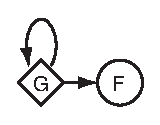
\includegraphics{nullmodel}
\end{center}

The G state has a symbol emission probability distribution for $K$
symbols in the alphabet. By default, this distribution is set either
to the average amino acid composition of SWISSPROT 34, or to 0.25 for
each nucleotide. The G $\rightarrow$ G transition controls the
expected length of observed random sequences; in practice, this
transition probability is so close to 1 that it has very little
effect. (It is set to 350/351 for protein models, 1000/1001 for DNA
models.) The F state is just a dummy end state like the T state in the
Plan 7 architecture.

The score of residues $x$ in match or insert states are:
\[
  s_x = \frac{p_x}{g_x}
\]

where $p_x$ is the probability according to the HMM, and $g_x$ is the
probabilitity according to the null model. Transition scores are also
calculated as log odds parameters. For details, see the source
documentation in \prog{plan7.c:P7Logoddsify()}.

As with the priors, copies of the default null model parameters are
provided, in the files \prog{tutorial/amino.null} and
\prog{tutorial/nucleic.null}.

Alternative null model files may be provided using the \prog{--null
<f>} option to \prog{hmmbuild}.

\subsection{Setting the alignment mode}

The model is then configured in one of four different alignment modes,
as described above. The default is hmmls mode: global with respect to
the model, multihit-local in the target sequence(s). The other modes
are selected with options:
\begin{enumerate}
\item[\prog{-f}] hmmfs, ``fragment'' mode: local in model,
multihit-local in sequence.
\item[\prog{-g}] hmms, ``global'' mode: global in model,
single hit global in sequence.
\item[\prog{-s}] hmmsw, ``Smith/Waterman'' mode: local in model,
single hit local in sequence.
\end{enumerate}

\subsection{Naming and saving the HMM}

HMM files have names (enabling them to be used in multi-HMM databases
for hmmpfam, like Pfam). The name must be one word, containing
no whitespace. The name is obtained in one of three ways:

\begin{itemize}
\item if a name \prog{<s>} is explicitly provided by the \prog{-n <s>}
      option, that's the name;
\item else if the alignment has a name (Stockholm \verb+#=GF ID+ or
      SELEX \verb+#=ID+ annotation), that's the name;
\item else the name is constructed by stripping off any suffix
      from the alignment file name. For instance, the alignment file
      ``rrm.phylip'' would result in an HMM named ``rrm''.
\end{itemize}
      
Finally, the HMM is saved. The default is to save it to the file named
on the \prog{hmmbuild} command line in a flat text, readable ASCII
format (page~\pageref{section:savefiles}. If the file already exists,
HMMER refuses to overwite it unless the \prog{-F} option was used to
force the overwrite, or the \prog{-A} option was used, which appends
to an existing HMM file rather than making a new HMM file.

A more space-efficient but undocumented binary format is available,
selected with the \prog{--binary} option. (Do not append binary HMMs
to ASCII files or vice versa; the program doesn't check to be sure
you're not doing this.) Minor but significant speed gains can be
obtained by working with large HMM databases in binary
format. Usually, one would convert an entire database to binary at
once, using the \prog{hmmconvert} program.




